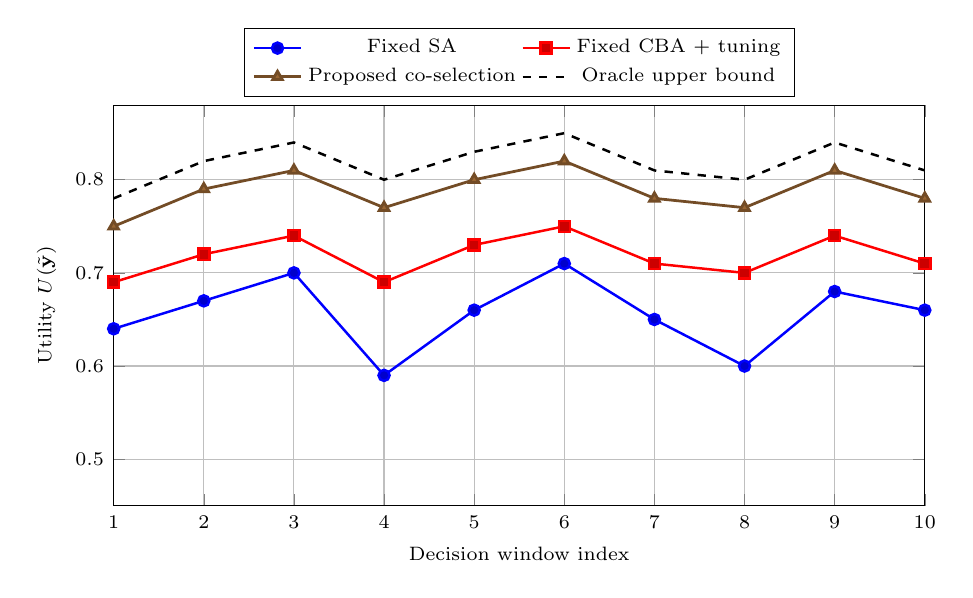
\begin{tikzpicture}
\begin{axis}[
  width=0.98\columnwidth,
  height=0.55\columnwidth,
  xmin=1, xmax=10,
  ymin=0.45, ymax=0.88,
  xlabel={Decision window index},
  ylabel={Utility $U(\tilde{\mathbf{y}})$},
  legend style={font=\scriptsize, at={(0.5,1.02)}, anchor=south, legend columns=2},
  grid=both,
  tick label style={font=\scriptsize},
  label style={font=\scriptsize}
]
\addplot+[mark=*, line width=0.9pt] coordinates {(1,0.64)(2,0.67)(3,0.70)(4,0.59)(5,0.66)(6,0.71)(7,0.65)(8,0.60)(9,0.68)(10,0.66)};
\addlegendentry{Fixed SA}

\addplot+[mark=square*, line width=0.9pt] coordinates {(1,0.69)(2,0.72)(3,0.74)(4,0.69)(5,0.73)(6,0.75)(7,0.71)(8,0.70)(9,0.74)(10,0.71)};
\addlegendentry{Fixed CBA + tuning}

\addplot+[mark=triangle*, line width=1.0pt] coordinates {(1,0.75)(2,0.79)(3,0.81)(4,0.77)(5,0.80)(6,0.82)(7,0.78)(8,0.77)(9,0.81)(10,0.78)};
\addlegendentry{Proposed co-selection}

\addplot+[mark=none, dashed, line width=0.9pt] coordinates {(1,0.78)(2,0.82)(3,0.84)(4,0.80)(5,0.83)(6,0.85)(7,0.81)(8,0.80)(9,0.84)(10,0.81)};
\addlegendentry{Oracle upper bound}
\end{axis}
\end{tikzpicture}
